% Option "table" is needed for xcolor package.
\documentclass[mathserif,table]{gkibeamer-aaai}

\usepackage{algorithm}
\usepackage[noend]{algpseudocode}
\usepackage{booktabs}
\usepackage{colortbl}
\usepackage{etex}  % Prevents "No room for a new \dimen" error.
\usepackage[utf8]{inputenc}
\usepackage{mathtools}
\usepackage[mode=buildnew]{standalone}
\usepackage{stmaryrd}
\usepackage{multicol}
\usepackage{xskak} % chessboard

\usepackage{pgfplots}
\usetikzlibrary{plotmarks}
\pgfplotsset{compat=1.9}

\usepackage {tikz}
\usepackage{pgfplots}
\usetikzlibrary {positioning}
\usepackage{tikz-cd}
\usetikzlibrary{arrows.meta,
chains,
positioning,
shapes.geometric, 
automata
}

\usepackage{todonotes}

\newcommand{\hilite}{\textcolor{structure}}
\newcommand{\blue}[1]{\textcolor{blue}{#1}}

%%% Abbreviations
\newcommand{\ie}{i.e.}
\newcommand{\eg}{e.g.}

%%% Definitions, theorems, and algorithms
\newcommand{\defined}[1]{\textbf{#1}}

\newcommand{\best}[1]{\textbf{\alert{#1}}}
\newcommand\weight[1]{\ensuremath{w(\text{#1})}}

%%% Mathematical symbols etc.
\newcommand{\pre}{\textit{pre}}
\newcommand{\eff}{\textit{eff}}
\newcommand{\cost}{\textit{cost}}
\newcommand{\post}{\textit{post}}
\newcommand{\varset}{\textit{varset}}
\newcommand{\sasplus}{\ensuremath{\textrm{SAS}^+}}
\newcommand{\astar}{\ensuremath{\textrm{A}^*}}
\newcommand{\Fact}[2]{\ensuremath{\langle #1, #2\rangle}}
\newcommand{\potential}{\ensuremath{\varphi}}
\newcommand{\hpot}[1]{\ensuremath{h_{#1}^{\potential}}}

\newcommand{\includefigure}[2][tbp]{
  \begin{figure}[#1]
    \centering
    \noindent
    \input{#2}
  \end{figure}
}

\newcommand{\includepicture}[4][tbp]{
  \begin{figure}[#1]
    \centering
    \noindent
    \includegraphics[width=#4]{#2}
    \caption*{#3}
    \label{figure:#2}
  \end{figure}
}


%%% Measures
\newcommand{\CC}{\textup{CC}}
\newcommand{\RM}{\textup{RM}}
\newcommand{\NW}{\textup{NW}}
\newcommand{\eNW}{\textup{eNW}}
\newcommand{\oNW}{\textup{oNW}}

\newcommand{\xDrawRod}[6]{% basex, basey, width, height, length, labelOut xDrawRod{2cm}{5cm}{3cm}{1cm}{9cm}{yes}{no}
	\draw[dashed] (#1,#2) arc (0:180: #3 and #4);
	\draw[] (#1,#2) arc (360:180: #3 and #4);
	\draw (#1,#2) -- (#1,#2 + #5);
	\draw (#1-#3-#3,#2) -- (#1-#3-#3,#2+#5);
	\node at (#1-#3,#2+#5*.5) {#6};
}

\newcommand{\xDrawCap}[6]{% basex, basey, width, height, length, labelOut xDrawRod{2cm}{5cm}{3cm}{1cm}{9cm}{yes}{no}
	\draw[] (#1,#2) arc (0:180: #3 and #4);
	\draw[] (#1,#2) arc (360:180: #3 and #4);
	\draw (#1,#2) -- (#1,#2 + #5);
	\draw (#1-#3-#3,#2) -- (#1-#3-#3,#2+#5);
	\node at (#1-#3,#2+#5*.5) {#6};
}

% Default itemize.
\setbeamertemplate{itemize items}[circle]

\setbeamertemplate{footline}
{
  \leavevmode%
  \hbox{%
  \begin{beamercolorbox}[wd=.3\paperwidth,ht=2.25ex,dp=1ex,center]{author in head/foot}%
    \usebeamerfont{author in head/foot}\insertshortauthor{~~(\insertshortinstitute)}
  \end{beamercolorbox}%
  \begin{beamercolorbox}[wd=.5\paperwidth,ht=2.25ex,dp=1ex,center]{title in head/foot}%
    \usebeamerfont{title in head/foot}\insertshorttitle
  \end{beamercolorbox}%
  \begin{beamercolorbox}[wd=.2\paperwidth,ht=2.25ex,dp=1ex,center]{page number in head/foot}%
    \usebeamerfont{page number in head/foot}\insertframenumber{} / \inserttotalframenumber
  \end{beamercolorbox}}%
  \vskip0pt%
}

% \setbeamercolor{page number in head/foot}{fg=white, bg=blue@AI!90!white}
% \setbeamerfont{page number in head/foot}{size=\footnotesize}

\title[Oxiflex - Constraint Programming Solver for MiniZinc]{Oxiflex - A Constraint Programming Solver for MiniZinc written in Rust}
\author[G.\ Klimmer]{Gianluca Klimmer}
\institute[unibas]{University of Basel}
\date{15.07.2024}
\subject{AI Planning}

% Needed for table overlays. See also
% http://www.math-linux.com/latex-26/article/how-to-make-a-presentation-with-latex-introduction-to-beamer
\setbeamercovered{invisible}

\usepackage{animate}
\usepackage{adjustbox}
\usetikzlibrary{positioning}

\begin{document}

\section{Rust}

\begin{frame}
	\only<1>{
		\begin{center}
			\LARGE{Constraint Programming Solver for MiniZinc written in Rust}
		\end{center}
	}
	\only<2>{
		\begin{center}
			\LARGE{Constraint Programming Solver for MiniZinc \textcolor{red}{written in Rust}}
		\end{center}
	}
\end{frame}

\begin{frame}{Rust}
	\begin{figure}[ht]
		
\includegraphics[scale=0.6]{./figures/rust_logo.png}
	\end{figure}
\end{frame}

\begin{frame}{Why Rust?}
	\begin{itemize}
		\item Performance
		      \pause
		      \begin{itemize}
			      \item $\rightarrow$ no abstractions, no garbage collector, no JIT
		      \end{itemize}
	\end{itemize}
\end{frame}

\begin{frame}{Possible Languages}
	\begin{multicols}{2}
		\begin{figure}[ht]
			
\includegraphics[scale=0.3]{./figures/c_logo.png}
		\end{figure}
		\columnbreak
		\begin{figure}[ht]
			
\includegraphics[scale=0.2]{./figures/cpp_logo.png}
		\end{figure}
	\end{multicols}
\end{frame}

\begin{frame}{Why Rust?}
	\begin{itemize}
		\item Performance
		      \begin{itemize}
			      \item $\rightarrow$ no abstractions, no garbage collector, no JIT
		      \end{itemize}
		\item Correctness
		      \begin{itemize}
			      \item Prevent bugs
		      \end{itemize}
		      \pause
		\item Ease of use
		      \begin{itemize}
			      \item Library manager - Cargo
			            \pause
			      \item Functional - Haskell similarities
			            \pause
			      \item Enums
			            \pause
		      \end{itemize}
		\item Learn Rust
	\end{itemize}
\end{frame}

\section{Constraint Programming}

\begin{frame}
	\only<1>{
		\begin{center}
			\LARGE{\textcolor{black}{Constraint Programming Solver for MiniZinc }\textcolor{blue}{written in Rust}}
		\end{center}
	}
	\only<2>{
		\begin{center}
			\LARGE{\textcolor{red}{Constraint Programming} Solver for MiniZinc \textcolor{blue}{written in Rust}}
		\end{center}
	}
\end{frame}

\begin{frame}
	\begin{center}
		\LARGE{Constraint Network}
	\end{center}
\end{frame}

\begin{frame}{Constraint Network}
	\begin{itemize}
		\item Variables
		      \begin{itemize}
			      \item Values to choose from
		      \end{itemize}
		\item Constraints
		      \begin{itemize}
			      \item Rules for choosing values
		      \end{itemize}
	\end{itemize}
\end{frame}

\begin{frame}{Simple Example}
	\begin{multicols}{2}
		\large{Variables:} \\
		\vspace{0.5cm}
		\hspace{0.5cm}
		$\begin{aligned}
				 & w \in \{1, 2, 3, 4\} \\
				 & y \in \{1, 2, 3, 4\} \\
				 & x \in \{1, 2, 3\}    \\
				 & z \in \{1, 2, 3\}    \\
			\end{aligned}$

		\columnbreak

		\large{Constraints:} \\
		\vspace{0.5cm}
		\hspace{0.5cm}
		$\begin{aligned}
				 & w = 2 \cdot x \\
				 & w < z         \\
				 & y > z         \\
			\end{aligned}$
	\end{multicols}
\end{frame}

\begin{frame}{Constraint Programming}
	\hspace{2cm}
	var 1..4: w; \\
	\hspace{2cm}
	var 1..4: y; \\
	\hspace{2cm}
	var 1..3: x; \\
	\hspace{2cm}
	var 1..3: z; \\
	\vspace{0.35cm}
	\hspace{2cm}
	constraint w = 2 $\cdot$ x; \\
	\hspace{2cm}
	constraint w $<$ z; \\
	\hspace{2cm}
	constraint y $>$ z; \\

	\pause
	\vspace{0.35cm}
	\hspace{2cm}
	solve satisfy;

	\pause
	\vspace{0.35cm}
	\hspace{2cm}
	$\rightarrow$ MiniZinc!
\end{frame}

\section{MiniZinc}

\begin{frame}{MiniZinc}
	\begin{figure}[ht]
		
\includegraphics[scale=0.2]{./figures/minizinc_logo.png}
	\end{figure}
	\begin{figure}[ht]
		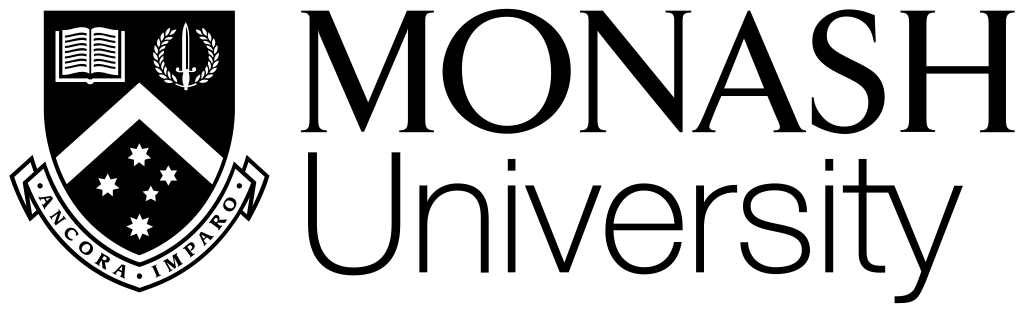
\includegraphics[scale=0.1]{./figures/monash_logo.png}
	\end{figure}
\end{frame}

\begin{frame}
	\begin{multicols}{3}
		\begin{figure}[ht]
			
\includegraphics[scale=0.15]{./figures/mzn-icon.png}
		\end{figure}
		\columnbreak
		\begin{center}
			\large{compilation} \\
			\huge{$\rightarrow$}
		\end{center}
		\columnbreak
		\begin{figure}[ht]
			
\includegraphics[scale=0.15]{./figures/fzn-icon.png}
		\end{figure}
	\end{multicols}
\end{frame}


\begin{frame}{FlatZinc}
	\only<1>{
	\hspace{1cm}
	array [1..2] of int: x\_introduced\_2\_ = [1,-2]; \\
	\hspace{1cm}
	array [1..2] of int: x\_introduced\_3\_ = [1,-1]; \\
	\hspace{1cm}
	array [1..2] of int: x\_introduced\_4\_ = [-1,1]; \\
	\vspace{0.35cm}
	\hspace{1cm}
	var 2..4: w:: output\_var; \\
	\hspace{1cm}
	var 1..4: y:: output\_var; \\
	\hspace{1cm}
	var 1..3: x:: output\_var; \\
	\hspace{1cm}
	var 1..3: z:: output\_var; \\
	\vspace{0.35cm}
	\hspace{1cm}
	constraint int\_lin\_eq(x\_introduced\_2\_,[w,x],0); \\
	\hspace{1cm}
	constraint int\_lin\_le(x\_introduced\_3\_,[w,z],-1); \\
	\hspace{1cm}
	constraint int\_lin\_le(x\_introduced\_4\_,[y,z],-1); \\
	\vspace{0.35cm}
	\hspace{1cm}
	solve  satisfy;
	}
	\only<2>{
	\hspace{1cm}
	\textcolor{red}{array [1..2] of int: x\_introduced\_2\_ = [1,-2];} \\
	\hspace{1cm}
	array [1..2] of int: x\_introduced\_3\_ = [1,-1]; \\
	\hspace{1cm}
	array [1..2] of int: x\_introduced\_4\_ = [-1,1]; \\
	\vspace{0.35cm}
	\hspace{1cm}
	var 2..4: w:: output\_var; \\
	\hspace{1cm}
	var 1..4: y:: output\_var; \\
	\hspace{1cm}
	var 1..3: x:: output\_var; \\
	\hspace{1cm}
	var 1..3: z:: output\_var; \\
	\vspace{0.35cm}
	\hspace{1cm}
	\textcolor{red}{constraint int\_lin\_eq(x\_introduced\_2\_,[w,x],0);} \\
	\hspace{1cm}
	constraint int\_lin\_le(x\_introduced\_3\_,[w,z],-1); \\
	\hspace{1cm}
	constraint int\_lin\_le(x\_introduced\_4\_,[y,z],-1); \\
	\vspace{0.35cm}
	\hspace{1cm}
	solve  satisfy;
	}
\end{frame}

\begin{frame}{FlatZinc constraint example}
	\hspace{1cm}
	predicate \textcolor{red}{int\_lin\_eq}(array [int] of int: as,\\
	\hspace{4.2cm} array [int] of var int: bs,\\
	\hspace{4.2cm} int: c)
	\pause
	\vspace{0.6cm}
	\begin{equation*}
		c = \sum_{i} \text{as}[i] \cdot \text{bs}[i]
	\end{equation*}
	\pause
	\vspace{0.6cm}
	\begin{equation*}
		w = 2 \cdot x
	\end{equation*}
\end{frame}

\begin{frame}
	\hspace{1cm}
	array [1..2] of int: x\_introduced\_2\_ = [1,-2]; \\
	\hspace{1cm}
	... \\
	\hspace{1cm}
	constraint int\_lin\_eq(x\_introduced\_2\_,[w,x],0); \\

	\pause

	\begin{equation*}
		c = \sum_{i} \text{as}[i] \cdot \text{bs}[i]
	\end{equation*}
	\pause
	\begin{equation*}
		0 = \sum_{i} \text{x\_introduced\_2\_}[i] \cdot \text{[w,x]}[i]
	\end{equation*}
	\pause
	\begin{equation*}
		0 = \sum_{i} \text{[1,-2]}[i] \cdot \text{[w,x]}[i]
	\end{equation*}
	\pause
	\begin{equation*}
		0 = 1 \cdot w - 2 \cdot x
	\end{equation*}
	\pause
	\begin{equation*}
		w = 2 \cdot x
	\end{equation*}
\end{frame}

\begin{frame}
	\only<1>{
		\begin{center}
			\LARGE{\textcolor{blue}{Constraint Programming} Solver \textcolor{blue}{for MiniZinc written in Rust}}
		\end{center}
	}
	\only<2>{
		\begin{center}
			\LARGE{\textcolor{blue}{Constraint Programming} \textcolor{red}{Solver} \textcolor{blue}{for MiniZinc written in Rust}}
		\end{center}
	}
\end{frame}

\section{Backtracking}

\begin{frame}
	\begin{center}
		\huge{Backtracking}
	\end{center}
\end{frame}

\newcommand{\backtracking}[2]{
	\only<#1>{
		\begin{figure}[ht]
			\centering
			\includegraphics[scale=0.3]{./figures/backtracking/backtracking_#2.png}
		\end{figure}
	}
}

\begin{frame}{Backtracking Example}
	\backtracking{1}{1}
	\backtracking{2}{2}
	\backtracking{3}{3}
	\backtracking{4}{4}
	\backtracking{5}{5}
	\backtracking{6}{6}
	\backtracking{7}{final}
	\backtracking{8}{solution}
\end{frame}

\begin{frame}
	\only<1>{
		\begin{center}
			\huge{Kinda like search...}
		\end{center}
	}
	\only<2>{
		\begin{center}
			\huge{Can we do better?}
		\end{center}
	}
\end{frame}

\section{8-Queens Problem}

\begin{frame}
	\begin{center}
		\huge{8-Queens Problem}
	\end{center}
\end{frame}

\begin{frame}{Chessboard}
	\begin{figure}[ht]
		\centering
		\newchessgame
		\chessboard[clearboard, showmover=false]
	\end{figure}
\end{frame}

\begin{frame}{One Queen}
	\only<1>{
		\begin{figure}[ht]
			\centering
			\newchessgame
			\chessboard[
				setfen=8/8/8/8/3Q4/8/8/8 w - - 0 1,
				showmover=false
			]
		\end{figure}
	}
	\only<2>{
		\begin{figure}[ht]
			\centering
			\newchessgame
			\chessboard[
				setfen=8/8/8/8/3Q4/8/8/8 w - - 0 1,
				color=red!50,
				pgfstyle=color,
				markfields={a7,b6,c5,a4,b4,c4,a1,b2,c3,d8,d7,d6,d5,d5,d3,d2,d1,e5,f6,g7,h8,e4,f4,g4,h4,e3,f2,g1},
				showmover=false
			]
		\end{figure}
	}
\end{frame}

\begin{frame}{Two Queens}
	\only<1>{
		\begin{figure}[ht]
			\centering
			\newchessgame
			\chessboard[
				setfen=8/8/8/5Q2/3Q4/8/8/8 w - - 0 1,
				showmover=false
			]
		\end{figure}
	}
	\only<2>{
		\begin{figure}[ht]
			\centering
			\newchessgame
			\chessboard[
				setfen=8/8/8/8/3Q1Q2/8/8/8 w - - 0 1,
				opacity=0.5,
				color=red!50,
				pgfstyle=color,
				markfields={d4,f4},
				showmover=false
			]
		\end{figure}
	}
\end{frame}

\begin{frame}{N-Queens Problem}
	\begin{itemize}
		\item Scalable
		      \pause
		      \begin{itemize}
			      \item 8-Queens $\rightarrow$ N-Queens
			            \pause
			      \item $n \times n$ chessboard
			            \pause
			      \item $n$ Queens
		      \end{itemize}
	\end{itemize}
\end{frame}

\section{Improvements}

\begin{frame}
	\begin{center}
		\huge{Inference}
	\end{center}
\end{frame}

\begin{frame}
	\begin{center}
		\huge{Forward Checking}
	\end{center}
\end{frame}

\begin{frame}{Forward Checking Example}
	\only<1>{
		\begin{figure}[ht]
			\centering
			\newchessgame
			\chessboard[
				setfen=8/8/8/8/3Q4/8/8/8 w - - 0 1,
				showmover=false
			]
		\end{figure}
	}
	\only<2>{
		\begin{figure}[ht]
			\centering
			\newchessgame
			\chessboard[
				setfen=8/8/8/8/3Q4/8/8/8 w - - 0 1,
				color=blue!50,
				pgfstyle=color,
				markfields={a7,b6,c5,a4,b4,c4,a1,b2,c3,e5,f6,g7,h8,e4,f4,g4,h4,e3,f2,g1},
				showmover=false
			]
		\end{figure}
	}
\end{frame}

\begin{frame}
	\begin{center}
		\huge{Arc Consistency}
	\end{center}
\end{frame}

\begin{frame}{Arc Consistency Example}
	\only<1>{
		\begin{figure}[ht]
			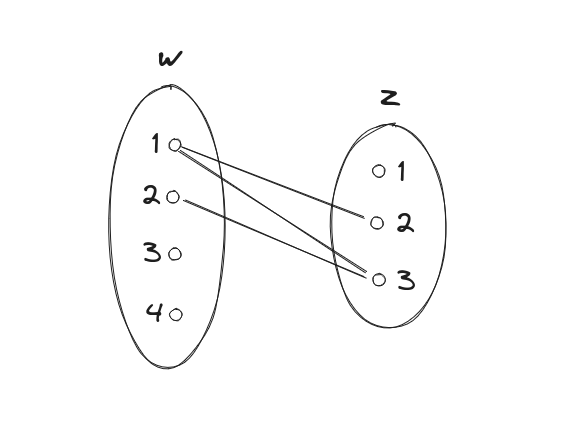
\includegraphics[scale=0.35]{./figures/arc_1.png}
		\end{figure}
	}
	\only<2>{
		\begin{figure}[ht]
			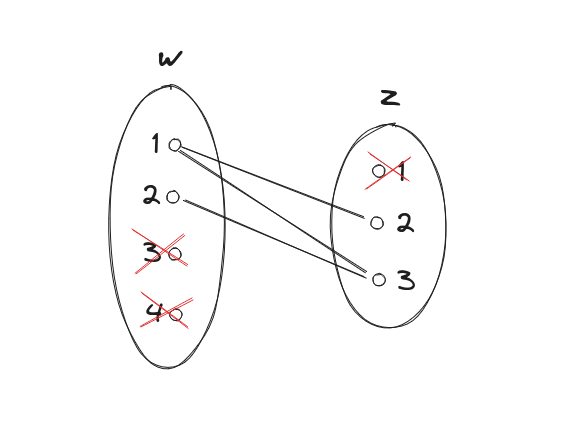
\includegraphics[scale=0.35]{./figures/arc_2.png}
		\end{figure}
	}
\end{frame}

\begin{frame}{Improvements}
	\begin{itemize}
		\item Inference
		      \pause
		      \begin{itemize}
			      \item Forward Checking
			            \pause
			      \item Arc consistency
			            \pause
			            \begin{itemize}
				            \item AC-1
				                  \pause
				            \item AC-3
			            \end{itemize}
			            \pause
		      \end{itemize}
		\item Dynamic Variable Ordering
	\end{itemize}
\end{frame}

\newcommand{\dyn}[2]{
	\only<#1>{
		\begin{figure}[ht]
			\centering
			\includegraphics[scale=0.3]{./figures/dyn_order/dyn_order_#2.png}
		\end{figure}
	}
}

\begin{frame}{Dynamic Variable Ordering}
	\dyn{1}{1}
	\dyn{2}{2}
	\dyn{3}{3}
	\dyn{4}{4}
\end{frame}

\section{Oxiflex}

\begin{frame}
	\only<1>{
		\begin{center}
			\huge{Oxiflex}
		\end{center}
	}
	\only<2>{
		\begin{center}
			\huge{Demo}
		\end{center}
	}
\end{frame}

\begin{frame}{Limitations}
	\begin{itemize}
		\item FlatZinc builtins
		      \pause
		      \begin{itemize}
			      \item IntLinEq
			      \item IntLinLe
			      \item IntLinNe
			            \pause
		      \end{itemize}
		\item No floating points
		      \pause
		\item No minimize / maximize
		      \pause
		\item Only one solution
	\end{itemize}
\end{frame}


\begin{frame}
	\begin{center}
		\LARGE{\textcolor{blue}{Constraint Programming Solver for MiniZinc written in Rust}}
	\end{center}
\end{frame}

\section{Benchmarks}

\begin{frame}
	\begin{center}
		\huge{Benchmarks}
	\end{center}
\end{frame}

\newcommand{\plot}[3]{
	\only<#1>{
		\begin{figure}[ht]
			\centering
			\includegraphics[scale=0.5]{./figures/plots/#2.png}
			\caption{#3}
		\end{figure}
	}
}

\begin{frame}
	\begin{center}
		\huge{N-Queens Problem}
	\end{center}
\end{frame}

\begin{frame}{Queens Time}
	\plot{1}{queens/time}{Averaged over $>10$ runs}
	\plot{2}{queens/time_no_arc}{Averaged over $>10$ runs}
\end{frame}

\begin{frame}{Queens Iterations}
	\plot{1}{queens/iterations}{Averaged over $5$ runs}
	\plot{2}{queens/iterations_inference}{Averaged over $5$ runs}
\end{frame}

\begin{frame}
	\begin{center}
		\huge{Slow Convergence}
	\end{center}
\end{frame}

\begin{frame}{Slow Convergence for small $n$}
	\plot{1}{slow/time_small}{Averaged over $>10$ runs}
	\plot{2}{slow/iterations_small}{Averaged over $5$ runs}
\end{frame}

\begin{frame}{Slow Convergence Comparison}
	\begin{multicols}{2}
		\begin{figure}[ht]
			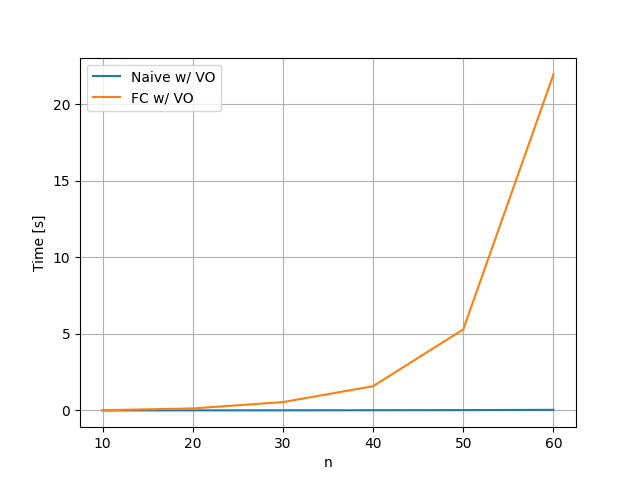
\includegraphics[scale=0.35]{./figures/plots/slow/time.png}
			\caption{Averaged over $>10$ runs}
		\end{figure}
		\columnbreak
		\begin{figure}[ht]
			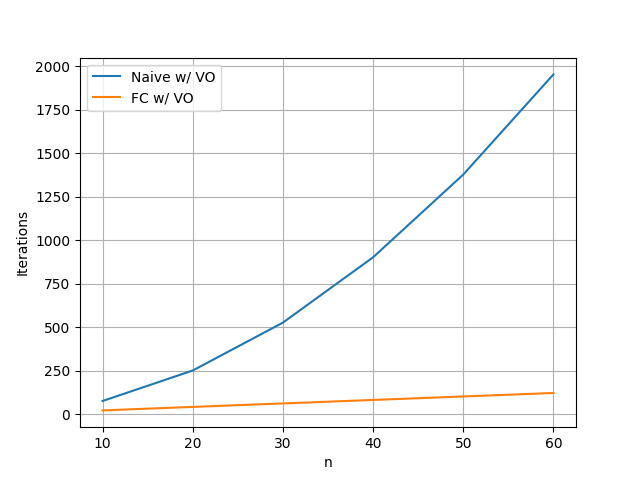
\includegraphics[scale=0.35]{./figures/plots/slow/iterations.png}
			\caption{Averaged over $5$ runs}
		\end{figure}
	\end{multicols}
\end{frame}

\begin{frame}{Oxiflex vs Gecode}
	\plot{1}{slow/gecode}{Averaged over $>10$ runs}
\end{frame}

\begin{frame}
	\begin{center}
		\huge{Conclusion}
	\end{center}
\end{frame}

\begin{frame}
	\begin{center}
		\huge{The end}
	\end{center}
\end{frame}

\end{document}
